\documentclass[12pt,a4paper]{report}
\usepackage[utf8]{inputenc}
\usepackage{amsmath}
\usepackage{amsfonts}
\usepackage{amssymb}
\usepackage{graphicx}
\usepackage{lmodern}
\usepackage{listings}
\usepackage[margin=0.5in]{geometry}

\author{Kyle Swanson}
\title{Chapter 6 Exercises: Architecture}

\setlength{\parindent}{0cm}

\begin{document}
\maketitle
\begin{normalsize}

\textbf{Exercise 6.4} - Repeat Exercise 6.3 for memory storage of a 32-bit word stored at memory word 15 in a byte-addressable memory. \\
a) What is the byte address of memory word 15? \\
$ 15 \times 4 = 15 \times 2^{2} = 1111 << 2 $ \\
$ = 111100 = 0x3C $ \\

b) What are the byte address that memory word 15 spans? \\
$ 0x3C to 111100 + 11 $ \\
$ = 111111 = 0x3F $ \\
$ 0x3C to 0x3F $ \\

c) Draw the number 0xFF223344 stored at word 15 in both big-endian and little-endian machines. Your drawing should be similar to Figure 6.4. Clearly label the byte address corresponding to each data byte value. \\
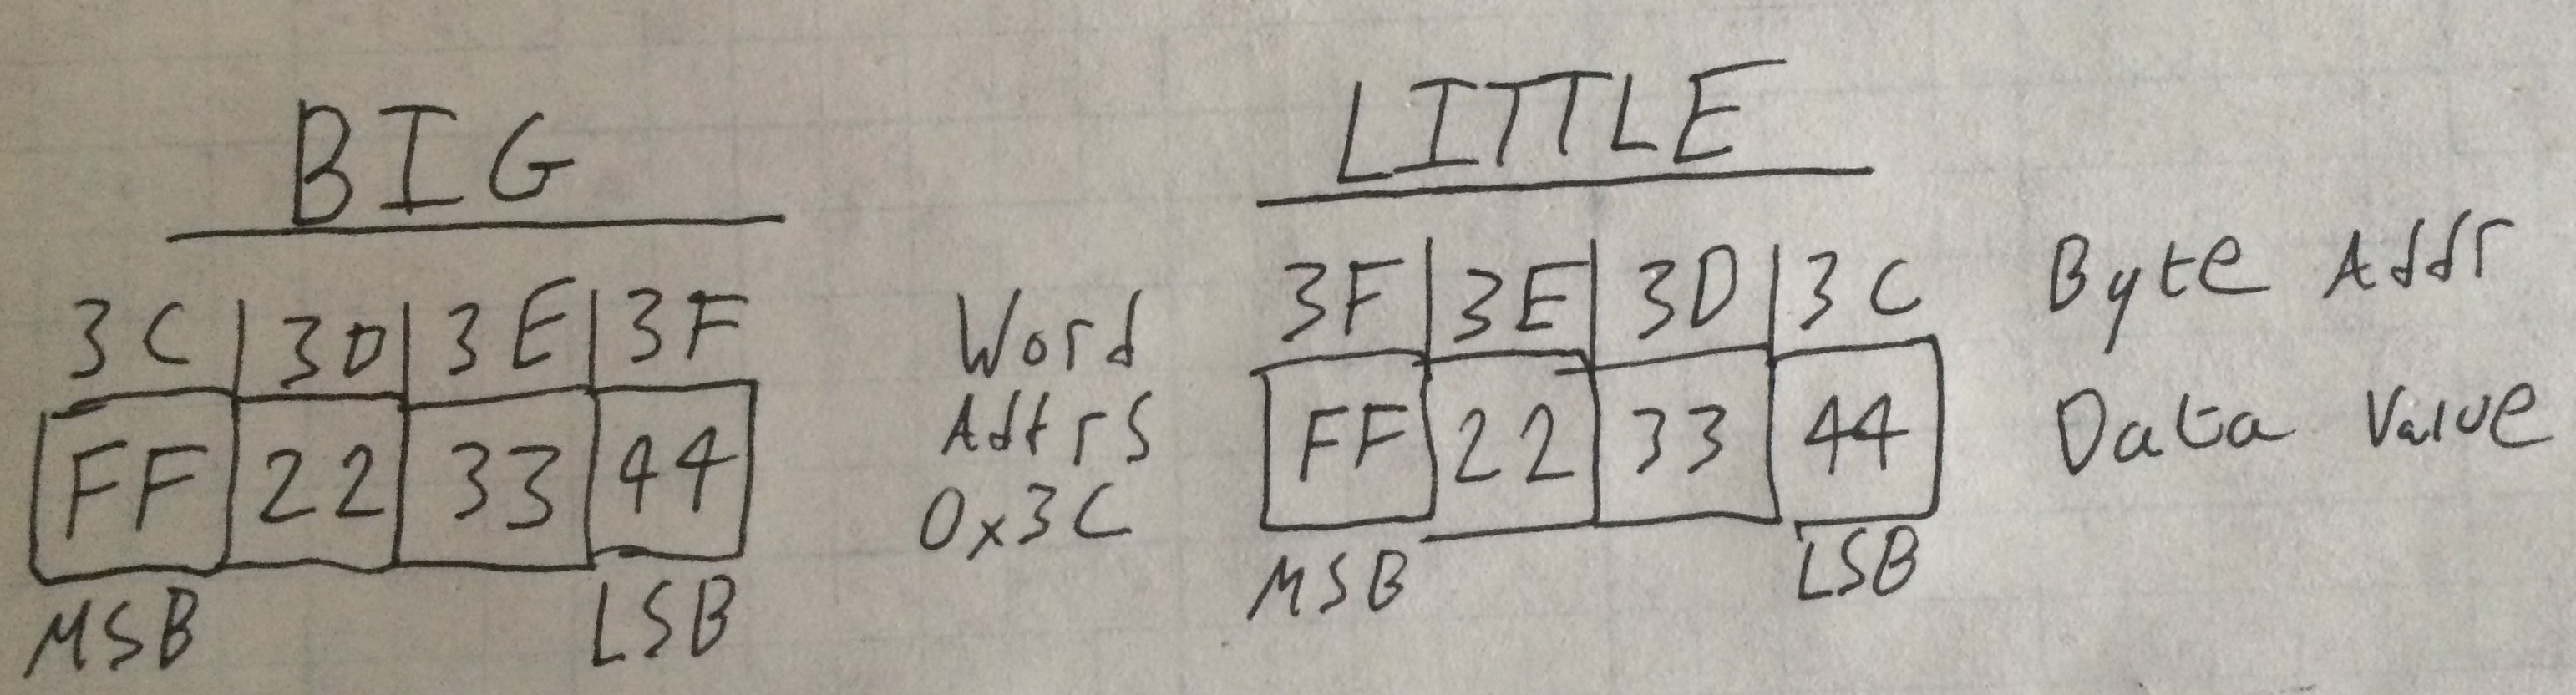
\includegraphics[scale=.15]{img/num} \\


\medskip

\textbf{Exercise 6.10} - Convert the following MIPS assembly code into machine language. Write the instructions in hexadecimal. \\
\textit{add \$t0, \$s0, \$s1} \\
This is an R-type instruction. Add \\
opcode = 000000 \\
rs = \$s0 = 16 = 10000 \\
rt = \$s1 = 17 = 10001 \\
rd = \$t0 = 8 = 01000 \\
shamt = 00000 \\
func = add = 100000 \\

Put it together: \\
000000 10000 10001 01000 00000 100000 \\
= \textbf{0x2114020} \\

\textit{lw \$t0, 0x20(\$t7)} \\
This is a I-type instruction. Load Word - lw rt, imm(rs) \\

opcode = 100011 \\
rs = \$t7 = 15 = 01111 \\
rt = \$t0 = 8 = 01000 \\
imm = 0x20 = 0000000000100000 \\

Put it together: \\
100011 01111 01000 0000000000100000 \\
= \textbf{0x8DE80020} \\

\textit{addi \$s0, \$0, -10} \\
This is a I-type instruction. Add Immediate - addi rt, rs, imm \\

opcode = 001000 \\
rs = 00000 \\
rt = 16 = 10000 \\
imm = -10 = 1111111111110110 \\

Put it together: \\
001000 00000 10000 1111111111110110 \\
= \textbf{0x2010FFF6} \\

\medskip

\textbf{Exercise 6.12} - Consider I-type instructions. \\
a) Which instructions from Exercise 6.10 are I-type instructions? \\
addi and lw are both I-type. \\

b) Sign-extend the 16-bit immediate of each instruction from part (a) so that it becomes a 32bit number. \\
lw immediate = 0000000000100000 \\
Sign extended = 0000000000000000 0000000000100000 = 0x20

addi immediate = 1111111111110110 \\
Sign extended = 1111111111111111 1111111111110110 = 0xFFFFFFF6



\medskip

\textbf{Exercise 6.14 - Do not complete the reverse engineering. Do not explain function. Just convert.} \\

0x20080000 = 001000 00000 01000 0000000000000000 \\
I-type \\
opcode = 001000 = addi \\
rs = 00000 = \$0 \\
rt = 01000 = \$t0 \\
imm = 0000000000000000 = 0 \\

addi \$t0, \$0, 0 \\

0x20090001 = 001000 00000 01001 0000000000000001 \\
I-type \\
opcode = 001000 = addi \\
rs = 00000 = \$0 \\
rt = 01001 = 9 = \$t1 \\
imm = 0000000000000001 = 1\\

addi \$t1, \$0, 1 \\ 

0x0089502A = 000000 00100 01001 01010 00000 101010 \\
R-type \\
opcode = 000000 \\
rs = 00100 = 4 = \$a0 \\
rt = 01001 = 9 = \$t1 \\
rd = 01010 = 10 = \$t2 \\
shamt = 00000 = 0 \\
func = 101010 = slt \\

slt \$t2, \$a0, \$t1 \\

0x15400003 = 000101 01010 00000 0000000000000011 \\
I-type \\
opcode = 000101 = bne \\
rs = 01010 = 10 = \$t2 \\
rt = 00000 = \$0 \\
imm = 0000000000000011 = 3 = 0x3 \\

bne \$t2, \$0, 0x3 \\

0x01094020 = 000000 01000 01001 01000 00000 100000 \\
R-type \\
opcode = 000000 \\
rs = 01000 = 8 = \$t0 \\
rt = 01001 = 9 = \$t1 \\
rd = 01000 = 8 = \$t0 \\
shamt = 00000 = 0 \\
func = 100000 = add \\

add \$t0, \$t0, \$t1

0x21290002 = 001000 01001 01001 0000000000000010 \\
I-type \\
opcode = 001000 = addi \\
rs = 01001 = 9 = \$t1 \\
rt = 01001 = 9 = \$t1 \\
imm = 0000000000000010 = 2\\

addi \$t1, \$t1, 2 \\

0x08100002 = 000010 00000100000000000000000010 \\
opcode = 000010 = j \\
label = 00000100000000000000000010 = 0x100002 \\

j 0x100002 \\

0x01001020 = 000000 01000 00000 00010 00000 100000 \\
R-type \\
opcode = 000000 \\
rs = 01000 = 8 = \$t0 \\
rt = 00000 = 0 = \$0 \\
rd = 00010 = 2 = \$v1  \\
shamt = 00000 = 0 \\
func = 100000 = add \\

add \$v1, \$t0, \$0 \\

0x03E00008 = 000000 11111 00000 00000 00000 001000 \\
R-type \\
R-type = opcode, rs, rt, rd, shamt, func
opcode = 000000 \\
rs = 11111 = 31 = \$ra \\
rt = 00000 = 0 = \$0 \\
rd = 00000 = 0 = \$0 \\
shamt = 00000 = 0 = \$0 \\
func = 001000 = jr \\

jr \$ra \\

\medskip

\textbf{Exercise 6.16} - The nori instruction is not part of the MIPS instruction set, because the same functionality can be implemented using existing functions. Write a short assembly code snippet that has the following functionality: \$t0 = \$t1 NOR 0xF234. Use as few instructions as possible. \\



\textbf{ARM Assignment Portion} \\
Please excuse the use of ^^ to denote a comment about the assembly code. \\
It seemed like the most clear/obvious way. \\

\textbf{1 - If} \\

\lstset{language=C}
\begin{lstlisting}
int main() {
    int counter = 0;

	if (counter == 1) {
		counter = 10;
	}

    return 0;
}
\end{lstlisting}	
\begin{center}
\small{A C language If loop.}
\end{center}

\lstset{language=[x86masm]Assembler}
\begin{lstlisting}
main:
         0x7a: 0x2000         MOVS      R0, #0
         0x7c: 0x2801         CMP       R0, #1 
         ^^ Compare the counter to 1. ^^
         0x7e: 0xd100         BNE.N     ??main_0                ; 0x82 
         ^^ Skip the if, if these are not equal. Branch to ??main_0 ^^
         0x80: 0x200a         MOVS      R0, #10                 ; 0xa
         ^^ if (counter == 1) do this line. ^^
??main_0:
         0x82: 0x2000         MOVS      R0, #0 
         ^^ Put 0 into the return register. ^^
         0x84: 0x4770         BX        LR
\end{lstlisting}	
\begin{center}
\small{A Assembler If loop}
\end{center}


\textbf{2 - If Else} \\

\lstset{language=C}
\begin{lstlisting}
int main() {
    int counter = 0;

	if (counter == 1) {
		counter = 10;
	} else {
		counter = 20;
	}

    return 0;
}
\end{lstlisting}	
\begin{center}
\small{A C language If Else loop.}
\end{center}

\lstset{language=[x86masm]Assembler}
\begin{lstlisting}
main:
         0x82: 0x2000         MOVS      R0, #0
         0x84: 0x2801         CMP       R0, #1 
         ^^ Compare counter to 1. The if statement. ^^
         0x86: 0xd101         BNE.N     0x8c 
         ^^ if counter isnt equal to 1. Go to the else. ^^
         0x88: 0x200a         MOVS      R0, #10                 ; 0xa
         ^^ Set counter to 10 if it was 1 ^^
         0x8a: 0xe000         B.N       0x8e
         0x8c: 0x2014         MOVS      R0, #20  ; 0x14 
         ^^ This is the else portion. ^^
         0x8e: 0x2000         MOVS      R0, #0
         0x90: 0x4770         BX        LR
\end{lstlisting}	
\begin{center}
\small{A If Else in Assembler}
\end{center}


\textbf{3 - Switch Case} \\

\lstset{language=C}
\begin{lstlisting}
int main() {
    int counter = 0;
    int a = 0;

    while (1) {
	switch (counter) {
		case 0:
                    a = 1;
                    break;
        case 1:
                    a = 2;
		case 2:
                    a = 3;
                    break;
		default:
                    return 0;
	}
        counter++;
    }
}
\end{lstlisting}	
\begin{center}
\small{A Switch Case in C Language}
\end{center}

\lstset{language=[x86masm]Assembler}
\begin{lstlisting}
main:
         0x40: 0x2000         MOVS      R0, #0
         0x42: 0x2100         MOVS      R1, #0
         ^^ Set the counter and a ^^
         0x44: 0xe001         B.N       ??main_0                ; 0x4a
??main_1:
         0x46: 0x2101         MOVS      R1, #1
??main_2:
         0x48: 0x1c40         ADDS      R0, R0, #1
??main_0:
         0x4a: 0x2800         CMP       R0, #0
         ^^ See if counter == 0. The first Case ^^
         0x4c: 0xd0fb         BEQ.N     ??main_1                ; 0x46
         0x4e: 0x2802         CMP       R0, #2
         ^^ see if counter == 2. The case 2. ^^
         0x50: 0xd001         BEQ.N     ??main_3                ; 0x56
         0x52: 0xd202         BCS.N     ??main_4                ; 0x5a
??main_5:
         0x54: 0x2102         MOVS      R1, #2
??main_3:
         0x56: 0x2103         MOVS      R1, #3
         0x58: 0xe7f6         B.N       ??main_2                ; 0x48
??main_4:
         0x5a: 0x2000         MOVS      R0, #0
         0x5c: 0x4770         BX        LRs
\end{lstlisting}	
\begin{center}
\small{A Switch Case in Assembler}
\end{center}


\textbf{4 - While} \\

\lstset{language=C}
\begin{lstlisting}
int main() {
    int counter = 0;

    while (counter < 10) {
        ++counter;
    }

    return 0;
}
\end{lstlisting}	
\begin{center}
\small{A While loop in the C language}
\end{center}

\lstset{language=[x86masm]Assembler}
\begin{lstlisting}
main:
         0x82: 0x2000         MOVS      R0, #0
         ^^ Set counter to 0 ^^
         0x84: 0xe000         B.N       0x88
         ^^ Skip this next instruction. Go to 0x88 ^^
         0x86: 0x1c40         ADDS      R0, R0, #1
         0x88: 0x280a         CMP       R0, #10                 ; 0xa
         ^^ Check if counter == 10 ^^
         0x8a: 0xdbfc         BLT.N     0x86
         ^^ if it's less than, go to 0x86. This is the while. ^^
         0x8c: 0x2000         MOVS      R0, #0
         0x8e: 0x4770         BX        LR
\end{lstlisting}	
\begin{center}
\small{A While loop in Assembler}
\end{center}


\textbf{5 - For} \\

\lstset{language=C}
\begin{lstlisting}
int main() {
    int counter = 0;

    for (int i=0; i<10; i++) {
        counter++;
    }

    return 0;
}
\end{lstlisting}	
\begin{center}
\small{A For Loop in the C Language}
\end{center}

\lstset{language=[x86masm]Assembler}
\begin{lstlisting}
main:
         0x7a: 0x2000         MOVS      R0, #0
         0x7c: 0x2100         MOVS      R1, #0
         ^^ Set counter and i to 0 ^^
         0x7e: 0xe001         B.N       ??main_0                ; 0x84
??main_1:
         0x80: 0x1c40         ADDS      R0, R0, #1
         0x82: 0x1c49         ADDS      R1, R1, #1
         ^^ Increment both i and counter ^^
??main_0:
         0x84: 0x290a         CMP       R1, #10                 ; 0xa
         ^^ Check if i is 10.
         0x86: 0xdbfb         BLT.N     ??main_1                ; 0x80
         ^^ If its less than, go back up. This is the for loop ^^         
         0x88: 0x2000         MOVS      R0, #0
         0x8a: 0x4770         BX        LR
\end{lstlisting}	
\begin{center}
\small{A For Loop in Assembler}
\end{center}


\textbf{6 - Array} \\

\lstset{language=C}
\begin{lstlisting}
int main() {
    int volatile array[5];

    for (int i=0; i<5; i++) {
        array[i] = i;
    }

    return 0;
}
\end{lstlisting}	
\begin{center}
\small{An array in the C language}
\end{center}

\lstset{language=[x86masm]Assembler}
\begin{lstlisting}
main:
         0x82: 0xb085         SUB       SP, SP, #0x14
         ^^ Allocate the array ^^
         0x84: 0x2000         MOVS      R0, #0
         0x86: 0xe003         B.N       0x90
         0x88: 0xa900         ADD       R1, SP, #0x0
         0x8a: 0xf841 0x0020  STR.W     R0, [R1, R0, LSL #2]
         ^^ Add i into the array ^^
         0x8e: 0x1c40         ADDS      R0, R0, #1
         0x90: 0x2805         CMP       R0, #5
         0x92: 0xdbf9         BLT.N     0x88
         ^^ Same deal, go back up if the loop should go ^^
         0x94: 0x2000         MOVS      R0, #0
         0x96: 0xb005         ADD       SP, SP, #0x14
         ^^ Overwrite the array? ^^
         0x98: 0x4770         BX        LR
\end{lstlisting}	
\begin{center}
\small{An array in Assembler}
\end{center}


\textbf{7 - Function Call} \\

\lstset{language=C}
\begin{lstlisting}
int main() {
    int counter = 0;
    int a = 1;
    int b = 2;
    int c = 3;
    int d = 4;
    int e = 5;
    int f = 6;

    while (counter < 5) {
        ++counter;
        int added = sum(counter, a, b, c, d, e, f);
    }

    return 0;
}

int sum(int counter, int a, int b, int c, int d, int e, int f) {
    int sum = counter + a + b + c + d + e + f;
    return sum;
}
\end{lstlisting}	
\begin{center}
\small{A simple function call in C}
\end{center}

\lstset{language=[x86masm]Assembler}
\begin{lstlisting}
main:
         0x40: 0xe92d 0x47f0  PUSH.W    {R4-R10, LR}
         0x44: 0xb084         SUB       SP, SP, #0x10
         0x46: 0x2400         MOVS      R4, #0
         0x48: 0x2501         MOVS      R5, #1
         0x4a: 0x2602         MOVS      R6, #2
         0x4c: 0x2703         MOVS      R7, #3
         0x4e: 0xf05f 0x0804  MOVS.W    R8, #4
         0x52: 0xf05f 0x0905  MOVS.W    R9, #5
         0x56: 0xf05f 0x0a06  MOVS.W    R10, #6
         ^^ Allocate the initial data ^^
         0x5a: 0xe00c         B.N       ??main_0                ; 0x76
??main_1:
         0x5c: 0x1c64         ADDS      R4, R4, #1
         0x5e: 0xf8cd 0xa008  STR.W     R10, [SP, #0x8]
         0x62: 0xf8cd 0x9004  STR.W     R9, [SP, #0x4]
         0x66: 0xf8cd 0x8000  STR.W     R8, [SP]
         0x6a: 0x003b         MOVS      R3, R7
         0x6c: 0x0032         MOVS      R2, R6
         0x6e: 0x0029         MOVS      R1, R5
         0x70: 0x0020         MOVS      R0, R4
         0x72: 0xf000 0xf806  BL        sum                     ; 0x82
         ^^ Go to the sum section. The function call. 
??main_0:
         0x76: 0x2c05         CMP       R4, #5
         0x78: 0xdbf0         BLT.N     ??main_1                ; 0x5c
         ^^ Check the end condition ^^
         0x7a: 0x2000         MOVS      R0, #0
         0x7c: 0xb004         ADD       SP, SP, #0x10
         0x7e: 0xe8bd 0x87f0  POP.W     {R4-R10, PC}
sum:
         0x82: 0x1808         ADDS      R0, R1, R0
         0x84: 0x1810         ADDS      R0, R2, R0
         0x86: 0x1818         ADDS      R0, R3, R0
         0x88: 0x9900         LDR       R1, [SP]
         0x8a: 0x1808         ADDS      R0, R1, R0
         0x8c: 0x9901         LDR       R1, [SP, #0x4]
         0x8e: 0x1808         ADDS      R0, R1, R0
         0x90: 0x9902         LDR       R1, [SP, #0x8]
         0x92: 0x1808         ADDS      R0, R1, R0
         0x94: 0x4770         BX        LR
         ^^ Return to the LR register address ^^
\end{lstlisting}	
\begin{center}
\small{A complex function call in Assembler}
\end{center}



\end{normalsize}
\end{document}